{\small
\begin{longtblr}[
    label = tab:Submodellelemente,
    entry = Submodellelemente im Package Explorer nach \cite{SpezifikationPart1},
    caption = {Submodellelemente im Package Explorer}
  ]{
    colspec = {c l l X{l}},
    rowhead = 1,
    vline{1,3,4,5} = {-}{},
    vline{2} = {-}{},
    hline{1-16} = {-}{} ,
    row{1} = {bg=tableHeader}
    }
    \textbf{Icon} & \textbf{\makecell[l]{Submodel-\\Element}} & \textbf{Beschreibung} & \textbf{Typ}\\
    \raisebox{-0.3\height}{
\includegraphics{Bilder/ModellierungAAS/Icons/Blob.PNG}} & Blob & Binärdatei                                                                  & DataElement \\
    \raisebox{-0.3\height}{
\includegraphics{Bilder/ModellierungAAS/Icons/Capability.PNG}} & Capability & \makecell[l]{Fähigkeit eines Assets, etwas bewirken \\ zu können (ohne konkrete Umsetzung)}                                                            & \makecell[l]{Submodel-\\Element} \\
    \raisebox{-0.3\height}{
\includegraphics{Bilder/ModellierungAAS/Icons/Entity.PNG}}&Entity & \makecell[l]{Einzelne Komponente (Asset) innerhalb \\ einer übergeordneten AAS  }                                                             & \makecell[l]{Submodel-\\Element} \\
    \raisebox{-0.3\height}{
\includegraphics{Bilder/ModellierungAAS/Icons/File.PNG}}&\makecell[l]{File} & \makecell[l]{Verlinkte oder eingebettete Datei mit \\ eindeutigem MIME-Type}                                                                & DataElement \\
    \raisebox{-0.3\height}{
\includegraphics{Bilder/ModellierungAAS/Icons/MLP.PNG}}&\makecell[l]{Multi-\\Language-\\Property} & Property mit mehrsprachigen Inhalten                             & DataElement \\
    \raisebox{-0.3\height}{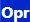
\includegraphics{Bilder/ModellierungAAS/Icons/Operation.PNG}}&Operation & \makecell[l]{Funktion mit Eingabe- und \\ Ausgabeparametern, die von einem System\\ ausgeführt werden kann}                                                              & \makecell[l]{Submodel-\\Element} \\
    \raisebox{-0.3\height}{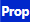
\includegraphics{Bilder/ModellierungAAS/Icons/Property.PNG}}&Property & Einfaches Merkmal mit festem Datentyp                   & DataElement  \\
    \raisebox{-0.3\height}{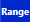
\includegraphics{Bilder/ModellierungAAS/Icons/Range.PNG}}&Range & Wertebereich mit Minimal- und Maximalwert                                                                  & DataElement\\
    \raisebox{-0.3\height}{
\includegraphics{Bilder/ModellierungAAS/Icons/RelationshipElement.PNG}}&\makecell[l]{Reference-\\Element} & Verweis auf interne oder externe Elemente                                     & DataElement \\
    \raisebox{-0.3\height}{
\includegraphics{Bilder/ModellierungAAS/Icons/Reference.PNG}}&\makecell[l]{Relationship-\\Element} & \makecell[l]{Beziehung zwischen zwei Elementen \\(sowohl intern als auch extern möglich)}                                  & \makecell[l]{Submodel-\\Element} \\
    \raisebox{-0.3\height}{
\includegraphics{Bilder/ModellierungAAS/Icons/SML.PNG}}&\makecell[l]{Submodel-\\ElementList} & \makecell[l]{Geordnete Liste verschiedener \\Submodellelemente}                                & \makecell[l]{Submodel-\\Element} \\
    \raisebox{-0.3\height}{
\includegraphics{Bilder/ModellierungAAS/Icons/SMC.PNG}}&\makecell[l]{Submodel-\\Element-\\Collection} & Sammlung von Submodellelementen                          & \makecell[l]{Submodel-\\Element} \\
\end{longtblr}
}